\section{Margaret (Dooley) (Simonds) Fernald}

\MainPerson{Margaret\textsuperscript{3} Dooley} (\Lineage{2}{Abigail}, \Lineage{1}{William}) was born in Watergrasshill, County Cork, Ireland, 27 December 1840.\cite{Margaret3DooleyBaptism} She died in Boston, Suffolk County, Massachusetts, 1 March 1918.\cite{Margaret3DooleyDeath} She married, first, probably between 1855--1860, \MainPerson{William Simonds},\cite{WilliamSimondsMarriage} and second, on 21 August 1873, \MainPerson{Ro\-bert A.\ Fer\-nald}\cite{RobertFernaldMarriage} (aka Robert A.\ Ireland).\cite{Census1855RobertFernald} William Simonds was born in Ireland about 1841\cite{Census1855WilliamSimonds} to Nicholas Simonds and Catharine (Keenan) Simonds.\cite{WilliamSimondsDeath,CatharineSimondsDeath} Robert A.\ Fernald was born in Boston about 1849 to George Fernald and Joanna (Whidhent) Fernald.\cite{RobertFernaldMarriage,JoannaFernaldDeath} He died in Boston on 14 June 1917.\cite{RobertFernaldDeath}

Margaret arrived in Boston on 27 June 1851, traveling with her mother, sister, and other relatives.\cite{Chascay}

Margaret's second husband, Robert A.\ Fernald, was a tugboat captain who ran the New England Dredging Company fleet.\cite{RobertFernaldDeath} Sometime between 1855 and 1860 Robert's family started using the surname ``Fernald'' instead of ``Ireland.''\cite{Census1855RobertFernald,Census1860RobertFernald}

\begin{figure}
	\centering
	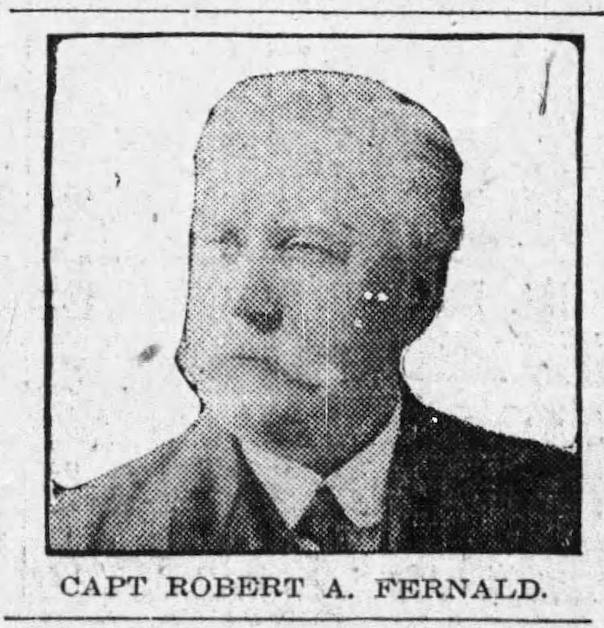
\includegraphics[width=0.5\textwidth]{fernald}
	\caption{Captain Robert A.\ Fernald. ``Robert A.\ Fernald, Veteran Tow Boat Captain, Dead,'' \textit{The Boston Globe}, 15 Jun 1917, p.\ 15.}
\end{figure}

\begin{KidsIntro}
	Children of William Simonds and Margaret\textsuperscript{3} (Dooley) Simonds:
\end{KidsIntro}

\begin{Kids}
	
	\KidNum{\ref{per:Catharine4Simonds}}{i.}\KidName{Catharine\textsuperscript{4} Simonds}, b.\ 19 Dec.\ 1860; m.\ 7 April 1879, \KidName{John McCarthy}.
	
	\KidNum{}{ii.}\KidName{Francis Simonds}, b.\ 4 June 1863;\cite{Francis4SimondsBirth} d.\ 27 June 1865.\cite{Francis4SimondsDeath}
	
	\KidNum{}{iii.}\KidName{Margaret Josephine Simonds}, b.\ 10 Aug.\ 1865;\cite{Margaret4SimondsBirth} d.\ 24 July 1866.\cite{Margaret4SimondsDeath}
	
	\KidNum{\ref{per:Abigail4Simonds}}{iv.}\KidName{Abigail J.\ Simonds}, b.\ 23 Jan.\ 1867; m.\ 13 April 1890, \KidName{John H.\ Rogan}.

\end{Kids}
	
\begin{KidsIntro}
	Children of Robert A.\ Fernald and Margaret\textsuperscript{3} (Dooley) (Simonds) Fernald:
\end{KidsIntro}	

\begin{Kids}
	
	\KidNum{}{v.}\KidName{Anna Fernald}, b.\ 25 June 1874;\cite{Anna4FernaldBirth} d.\ 5 May 1875.\cite{Anna4FernaldDeath}
	
	\KidNum{\ref{per:Caroline4Fernald}}{vi.}\KidName{Caroline Emma Fernald}, b.\ 16 March 1876; m.\ 19 Oct.\ 1893, \KidName{John Joseph McGurin}.
		
	\KidNum{\ref{per:Sarah4Fernald}}{vii.}\KidName{Sarah Helen Fernald}, b.\ 5 March 1879; m.\ 30 Sept.\ 1902, \KidName{Christopher Leonard}.
	
	\KidNum{\ref{per:Robert4Fernald}}{viii.}\KidName{Robert Atwell Fernald}, b.\ 19 June 1882; m.\ 28 June 1911, \KidName{Agnes M.\ Leonard}. Agnes is the sister of Christopher Leonard, who married Robert's sister Sarah.
	
\end{Kids}
	
	
